\documentclass[border=3pt,tikz]{standalone}
% Shared look for every TikZ figure in these notes.
% Included by each standalone figure file; also keeps the figures consistent
% with the colours used in the PDF and on the website.

\usepackage{tikz}
\usepackage{pgfplots}
\pgfplotsset{compat=1.18}
\usetikzlibrary{arrows.meta, decorations.markings, decorations.pathmorphing,
                patterns, calc, positioning}
\usepackage{amsmath}

% Series colours are the three validated categorical slots also used by the
% interactive widgets, so a path drawn in the printed notes and the same path on
% the website are the same colour. They clear the colour-vision-deficiency and
% contrast checks as a set; every path is direct-labelled as well, so colour is
% never the only thing carrying identity.
\definecolor{duPurple}{HTML}{68246D}
\definecolor{duBlue}{HTML}{2A78D6}
\definecolor{duRed}{HTML}{EB6834}
\definecolor{duGreen}{HTML}{1BAF7A}
\definecolor{duGrey}{HTML}{6B6B6B}

\tikzset{
  axisline/.style   = {-{Stealth[length=3mm]}, line width=0.7pt, black},
  path1/.style      = {duBlue,   line width=1.1pt},
  path2/.style      = {duRed,    line width=1.1pt},
  path3/.style      = {duGreen,  line width=1.1pt},
  statedot/.style   = {circle, fill=black, inner sep=1.4pt},
  arrowhead/.style  = {decoration={markings,
                        mark=at position #1 with {\arrow{Stealth[length=2.6mm]}}},
                       postaction={decorate}},
  lbl/.style        = {font=\small},
  slbl/.style       = {font=\footnotesize, duGrey},
  workfill/.style   = {duPurple, opacity=0.16},
}

% irreversible (dashed): areas mean nothing; reversible: areas are |w| and |q|
\begin{document}
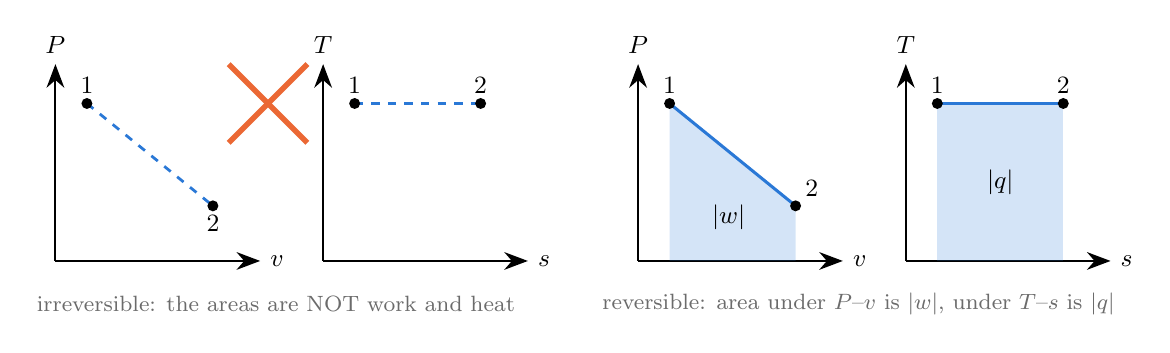
\begin{tikzpicture}[x=1cm,y=1cm]
  \newcommand{\ax}[3]{%
    \begin{scope}[shift={(#1,0)}]
      \draw[axisline] (0,0) -- (2.6,0) node[right, lbl] {$#3$};
      \draw[axisline] (0,0) -- (0,2.5) node[above, lbl] {$#2$};
    \end{scope}}
  % irreversible
  \ax{0}{P}{v}
  \draw[duBlue, dashed, line width=1pt] (0.4,2.0) -- (2.0,0.7);
  \node[statedot] at (0.4,2.0) {}; \node[lbl, above] at (0.4,2.0) {1};
  \node[statedot] at (2.0,0.7) {}; \node[lbl, below] at (2.0,0.7) {2};
  \ax{3.4}{T}{s}
  \draw[duBlue, dashed, line width=1pt] (3.8,2.0) -- (5.4,2.0);
  \node[statedot] at (3.8,2.0) {}; \node[lbl, above] at (3.8,2.0) {1};
  \node[statedot] at (5.4,2.0) {}; \node[lbl, above] at (5.4,2.0) {2};
  \draw[duRed, line width=2pt] (2.2,2.5) -- (3.2,1.5); \draw[duRed, line width=2pt] (2.2,1.5) -- (3.2,2.5);
  \node[slbl] at (2.8,-0.55) {irreversible: the areas are NOT work and heat};
  % reversible
  \ax{7.4}{P}{v}
  \fill[duBlue, opacity=0.2] (7.8,0) -- (7.8,2.0) -- (9.4,0.7) -- (9.4,0) -- cycle;
  \draw[path1] (7.8,2.0) -- (9.4,0.7);
  \node[statedot] at (7.8,2.0) {}; \node[lbl, above] at (7.8,2.0) {1};
  \node[statedot] at (9.4,0.7) {}; \node[lbl, above right] at (9.4,0.7) {2};
  \node[lbl] at (8.55,0.55) {$|w|$};
  \ax{10.8}{T}{s}
  \fill[duBlue, opacity=0.2] (11.2,0) rectangle (12.8,2.0);
  \draw[path1] (11.2,2.0) -- (12.8,2.0);
  \node[statedot] at (11.2,2.0) {}; \node[lbl, above] at (11.2,2.0) {1};
  \node[statedot] at (12.8,2.0) {}; \node[lbl, above] at (12.8,2.0) {2};
  \node[lbl] at (12.0,1.0) {$|q|$};
  \node[slbl] at (10.2,-0.55) {reversible: area under $P$--$v$ is $|w|$, under $T$--$s$ is $|q|$};
\end{tikzpicture}
\end{document}
